\documentclass[11pt,a4paper]{moderncv}

\usepackage[german]{babel}
\usepackage[utf8]{inputenc}
\usepackage{multicol}
\moderncvtheme[blue]{casual}
\usepackage{moderncv-additions}

% adjust the page margins
\usepackage[scale=0.8]{geometry}
\setlength{\hintscolumnwidth}{3cm}

\AtBeginDocument{\recomputelengths}

% personal data
\firstname{Philipp}
\familyname{Scholl}
\address{%
    16 An Tor Aonarach, Dunaree, %
    Kingscourt, Co. Cavan}{%
    A82 V2H0, Irland}%
\mobile{+49 152 020 95 226, +353 87 1922 755}
\email{rayleighsjeans@gmail.com}
\photo[64pt]{picture}

\newcommand{\sign}[1]{%
    \begin{tabular}[t]{@{}l@{}}
    \makebox[1.5in]{\dotfill}\\
    \strut\emph{#1}\strut%
    \end{tabular}}%
\newcommand{\position}{%
    Physiker KI-Algorithmen und hybriden Lösungen}%
\newcommand{\posaddress}{%
    MICHAEL GLAS IMMOBILIEN\\%
    Daiserstraße 41\\%
    81371 München\\%
    Deutschland}%

%  content
\begin{document}

    % color redefinitions must be after \begin{document}!
    % \definecolor{firstnamecolor}{RGB}{138,74,57}%
    \definecolor{firstnamecolor}{RGB}{0,50,95}%
    \definecolor{familynamecolor}{RGB}{0,50,95}%
    \definecolor{quotecolor}{RGB}{0,70,110}%
    \definecolor{addresscolor}{RGB}{0,70,110}%
    \definecolor{sectionrectanglecolor}{RGB}{0,50,95}%
    \definecolor{sectiontitlecolor}{RGB}{0,50,95}%
    \definecolor{subsectioncolor}{RGB}{0,70,110}%
    \definecolor{footersymbolcolor}{RGB}{0,70,110}%
    \definecolor{chaptertitlecolor}{RGB}{0,50,95}

    \makeatletter
    \pagestyle{empty}
    \chapter*{Curriculum Vitae}{}

    \vspace*{3.5cm}
    \begin{minipage}{\textwidth}
        \vspace*{3mm}
        \familynamestyle{\@firstname}~\familynamestyle{\@familyname}
            %\hfill%
            \hspace{10mm}
            {{\color{firstnamecolor}\includegraphics[width=96pt]%
                {../figures/images/52.png}}}\\[0.3cm]
            \@addressstreet\\[0.0cm]%
            \@addresscity\\[0.3cm]%
            \mobilesymbol~\@mobile\\[0.3cm]%
            \emailsymbol~\@email%
    \end{minipage}
    \begin{minipage}{70pt}
    \end{minipage}
    \vfill

    %  letter
    \newpage
    \makeatletter%
    % \chapter{Bewerbung}{}
    % \vspace*{1.0cm}
    % \begin{minipage}{0.6\textwidth}
    %     \begin{flushleft}
    %         \posaddress%
    %     \end{flushleft}
    % \end{minipage}
    % \hfill
    % \begin{minipage}{0.3\textwidth}
    %     \begin{flushright}
    %         \@firstname~\@familyname\\%
    %         \@addressstreet\\%
    %         \@addresscity%
    %     \end{flushright}
    % \end{minipage}

    % \vspace*{1.0cm}
    % {\bfseries \color{familynamecolor}%
    %     Bewerbung für: Michael Glas Immobilien, Betzenweg 20% TODO
    %     % Initiativbewerbung%
    % }\\[0.5cm]
%
    % Sehr geehrte Damen und Herren,\\[0.25cm]
%
    % Meine Partnerin Stella Scholl und ich möchten uns mit diesem Anschreiben kurz vorstellen und auf Ihre Wohnung im Betzenweg 20 bewerben.\\[0.25cm]%
%
    % Aktuell sind wir noch, einerseits als Krankenschwester im Intensivbereich am Uniklinikum Greifswald, und andererseits Promotionsstudent der Physik in den letzten Zügen am Max-Planck-Institut Greifswald beschäftig.\\[0.25cm]
%
    % Auf Grund einer Neuanstellung bei Krauss-Maffei Wegmann GmbH \& Co. KG meinerseits ziehen wir von der Ostsee nach München.\\[0.25cm]%
%
    % Wir sind ein junges, ruhiges Paar ohne Kinder. Zu uns gehören zwei, ca. 5 Jahre alte, stubenreine und kastriert Kater, die sicherlich nichts mehr glücklich machen würde als ein Balkon für die Vogelschau.\\[0.25cm]%
%
    % Die von Ihnen angebotene Wohnung, welche bereits durch Frau Scholl in persona besichtigt wurde, hat uns auf Anhieb gefallen und wir würden uns sehr über eine Mietvertragsangebot freuen.\\[0.25cm]%
%
    % Weiterhin würden wir uns über eine zeitnahe Rückmeldung, aber auch gerne über ein Angebot zum Gespräch, bei dem Sie uns einmal persönlich kennenlernen können, sehr freuen.\\%

    % hiermit möchte ich %
    % % Ihnen meine Initiativbewerbung zukommen lassen.\\[0.25cm]%
    % mich initial auf die Stelle eines\\\position~bewerben.\\[0.25cm]  % TODO
%
    % Momentan arbeite ich an meiner Doktorarbeit unter der Aufsicht von Prof. Dr. Thomas Klinger am Max-Planck Institut für Plasmaphysik in Greifswald. Diese werde ich voraussichtlich mit ihrer Einreichung und Verteidigung zwischen Mitte und Ende April 2021 abschließen.\\[0.25cm]%
%
    % Im Laufe meines Studiums und besonders meiner Promotion hatte ich die Möglichkeit, mir verschiedene Fähigkeiten in Bereichen der Steuerung, Optimierung und Integration von Software anzueignen. Insbesondere während meiner Promotion konnte ich Erfahrungen mit der Konzeptionierung, dem Design, der Kontrolle und Implementierung von Forward-Feedback Steuerungen machen. Während meiner Arbeit zur Promotion arbeitete ich an der zentralen Bolometrie im Stellarator Wendelstein 7-X und konzentrierte mich dabei speziell auf die Referenzierung dieser optischen Diagnostik.\\[0.25cm]%
%
    % Extensive Programmierkenntnisse und -erfahrungen habe ich besonders während meiner Masterarbeit in C++ Particle-in-Cell Simulationen von Plasmen sammeln können. Die vielfältige Datenauswertung und Modellierung von großen Datenmengen in Python und Simulationen in Fortran bzw. IDL sind aktuell zentraler Teil meiner Doktorarbeit.\\[0.25cm]%
%
    % Zur weiterführenden Ausbildung habe ich unter anderem während meiner Promotion die Vorlesung von Prof. M. Stanke zum Thema Maschinelles Lernen besucht, um dort meine praktischen Erfahrungen, die ich bei der Optimierung der PIC-Computersimulation gesammelt habe, mathematisch-theoretisch zu festigen.\\[0.25cm]%
%
    % Meine Neugierde und Passion für die intelligente Lösung von komplexen Problemen motoviert mich für die Bewerbung in einem Bereich mit neuen Herausforderungen.\\[0.25cm]%
%
    % Abschließend notiere ich Namen und Kontaktinformationen meiner früheren Vorgesetzten zur Referenz.\\[0.25cm]%
    % \hspace*{0.5cm}Prof. Dr. Andre Melzer (Kolloide Plasmen)%
    %     \hfill Tel. +49~3834~/~420~4790\\%
    % \hspace*{0.5cm}Prof. Dr. Ralf Schneider (Computational Science)%
    %     \hfill Tel. +49~3834~/~420~1400\\%
    % \hspace*{0.5cm}Prof. Dr. Thomas Klinger (E5 - Divertor-Dynamik und -Transport)%
    %     \hfill Tel. +49~3834~/~~\,88~2500\\%
%
    % \begin{flushleft}%
    %     Mit freundlichen Grüßen,\\%[0.25cm]
    %     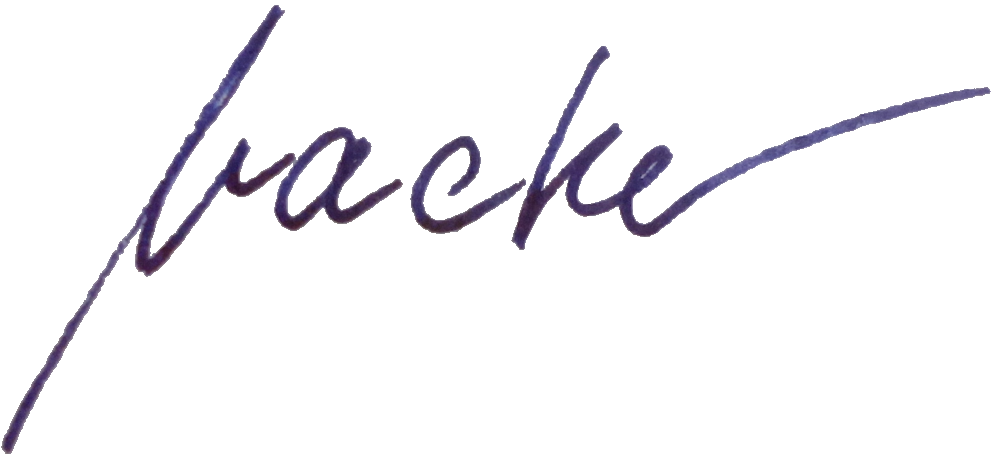
\includegraphics[width=3.0cm]{%
    %         ../figures/images/signature_transparent.png}
    %     \vspace*{-1.0cm}\hspace*{-3.0cm}%
    %     \sign{Philipp Hacker}\\%
    %     % Greifswald; \today
    % \end{flushleft}%
    % \newpage

    \pagestyle{fancy}
    \chapter{Curriculum}{~Vitae}
    \makequote%

    \section{Persönliche~Informationen}
    \cvline{Name}{\@firstname~\@familyname}
    \cvline{Adresse}{\@addressstreet\newline \@addresscity}
    \cvline{Telefon}{\@mobile}
    \cvline{eMail}{\@email}
    \cvline{Geburtsdatum}{15.~Juni,~1994~in~Demmin}
    \cvline{Nationalität}{Deutschland}
    \cvline{Familienstand}{verheiratet}
    \cvline{Geschlecht}{männlich}
    \makeatother

    \section{Sprachen}
    \cvline{Deutsch}{erste Sprache, Muttersprache}{}
    \cvline{Englisch}{zweite Sprache, erste Fremdsprache\newline%
        C2 Zertifikat, 7 Jahre Schulbildung}{}
    \cvline{Russisch}{dritte Sprache, zweite Fremdsprache\newline%
        5 Jahre Schuldbildung}{}

    \section{Schule}
    \cventry{08/2000~--~03/2004}{Grundschule}{%
        Grundschule~Jarmen\newline~Jarmen}{}{}{}
    \cventry{08/2004~--~08/2010}{Mittelstufe}{Regionale~Schule~Jarmen\newline~Jarmen}{}{}{}
    \cventry{08/2010~--~06/2012}{Gymnasialstufe}{%
        Schlossgymnasium Gützkow}{Gützkow}%
        {Hochschulreife}{}

    \section{Hochschulausbildung}
    \cventry{10/2012~--~09/2015}{Bachelorabschluss~in~Physik}{%
            Ernst-Moritz-Arndt~Universität}%
        {Greifswald}{Bachelor~of~Science}{%
        }
    \cventry{10/2012~--~10/2017}{Masterabschluss~in~Physik}{%
            Ernst-Moritz-Arndt~Universität}%
        {Greifswald}{Master~of~Sciences}{%
        }
    \cventry{11/2017~--~now}{doctor rerum naturalium~-~Physics}{%
        Max-Planck~Institut~für~Plasmaphysik}%
        {Greifswald}{}{}
        
    \section{Berufserfahrung}
        \cventry{07/2021 -- 04/2024}{Software-Entwickler - C/C++}{%
            Krauss-Maffei Wegmann Nexter Defense Systems}%
        {Munich}{Fortgeschrittenes C/C++, \textit{Embedded} Entwickling, Frameworks, APIs, AI, \textit{CGFs - computer generated forces}, Dynamik \& Simulator-Logik}{}%
        \cventry{11/2017 -- 05/2021}{Wissenschaftler/Doktorand - Plasmaphysik}{%
            Max-Planck Institut für Plasmaphysik}%
        {Greifswald}{Datenanalyse, Modelbildung, Simulation, Entwicklung von Embedded-Systemen}{}
        \cventry{12/2024 -- now}{Software-Entwicklung}{%
            IBM - International Business Machines Research Lab}%
        {Mulhuddart, Ireland}{Fortgeschrittenes C/C++ für Datenbank-Engine \textit{DB2}, Hybrid Data Management mit Fokus auf objecktorientierte LSM Cloud-Speicher; Regressions-Tests und QA, Leistungs-Benchmarks und Analyse-Tools}{}
        
    \subsection{Weiterbildungen}
        \cventry{02/2022}{Advanced C++ (for Embedded Systems)}{%
            MicroConsult Microelectronics Consulting \& Training GmbH}%
            {Munich}{Grundlagen, Muster, Idiome, Paradigmen, „modernes C++}{}
        \cventry{Jun.~2019}{Plan,~Motivate,~Achieve:~Time~and~Self-Management}{Transferable~Skills~Seminar}{R.~Thompson}{International~Helmholtz~Graduate~School~for~Plasma~Physics}{}
        \cventry{Jun.~2019}{Presentation~Skill~Workshop}{Transferable~Skills~Seminar}{B.~Hey}{International~Helmholtz~Graduate~School~for~Plasma~Physics}{}

    \section{Wissenschaftliche~Praxiserfahrung}
    \cventry{10/2012~--~04/2014}{Grundpraktikum,~Laborpraktikum}%
        {Grundlegende~Experimente~in~allen~Forschungsgebieten~im~Institut~für~Physik\newline}{}%
        {Universität~Greifswald}{}
    \cventry{05/2015~--~09/2015}{%
            Bachelorarbeit:~`Modenanregung~in~Yukawa-Bällen'}%
        {Arbeitsgruppe~Prof.~Dr.~Andre~Melzer\newline}{}%
        {Universität~Greifswald\newline}{Stereoskopische~Partikeldiagnostik~in~MATLAB}
    \cventry{10/2015~--~07/2016}{Praktikum~in~der~Arbeitsgruppe~von~Prof.~Dr.~Melzer}%
        {Komplexe~Plasma-Systeme,~experimenteller~Aufbau\newline}{}%
        {Institut~für~Physik,~Universität~Greifswald}{}
    \cventry{10/2015~--~04/2016}{Fortgeschrittenen-Praktikum}%
        {Fortgeschrittene~experimentelle~Methoden\newline}{}%
        {Institut~für~Physik,~Universität~Greifswald}{}
    \cventry{04/2016~--~10/2016}{Arbeitsgruppen-Praktikum}%
        {`Electric~field~strength~spectroscopy~in~dielectric~barrier~discharges'\newline}{}%
        {Arbeitsgruppe~Prof.~Dr.~Jürgen~Meichsner\newline}%
        {Institut~für~Physik,~Universität~Greifswald}
    \cventry{10/2016~--~10/2017}{%
        Master-Arbeit:~`Kinetic~Effects~in~RF~Discharges'}%
        {Arbeitsgruppe~Prof.~Dr.~Ralf~Schneider\newline}{}%
        {Institut~für~Physik,~Universität~Greifswald\newline}%
        {C++ 2d3v PIC Simulation von ccrf Entladungen}
    \cventry{11/2017~--~jetzt}{%
        Internationale~Helmholtz~Graduatierten-Schule~für~Plasma-Physik}%
        {Graduatierten-Schule~für~Promotionsstudenten~des~MPI~für~Plasma-Physik\newline}{}%
        {MPI~für~Plasma-Physik,~Greifswald;~Universität~Greifswald\newline}%
        {Präsentationen~in~und~Teilnahme~an~Kolloquia,~Workshops~und~Konferenzen}
    \cventry{11/2017~--~jetzt}{%
        Promotion:~`Impurity~radiation~and~transport~at~the~stellarator~W7-X'}%
        {Abteilung~für~Stellarator-Dynamik~und~-Transport,~Prof.~Dr.~T.~Klinger\newline}{}%
        {Max-Planck~Institut~für~Plasma-Physik,~Greifswald\newline}%
        {Echtzeit-Feedback~mit~Plasma-Strahlung,~Evaluierung~von~lokalen~Strahlungs-Effekten}

    \section{Lehrtätigkeiten}
    \cventry{03/2014~--~10/2018}{%
        Praktikums-Assistenz~im~Grundpraktikum~der~Physik}%
        {in:~Studienfach~der~Human-Medizin\newline}{}%
        {Institut~für~Physik,~Universität~Greifswald}{}

    \section{Publikationen}
        \cventry{May 2018}{`PIC Simulation of electronegative CCRF discharges'}{%
          Authors: P. Matthias, R. Schneider, J. Meichsner, G. Bandelow, J. Duras, K. Matyash, K.-F. Lüskow, D. Kahnfeld, S. Kemnitz, L. Lewerentz and P. Hacker}{
          doi: 10.1140/epjd/e2017-80565-y}{}{}{}
        \cventry{Dec. 2019}{`Measurement of edge ion temperature in W7-X with island divertor by retarding field analyzer'}{%
          Authors: Y. Li, T. Henkel, Y. Liang, A. Knieps, P. Drews, C. Killer, D. Nicolai, J. Cosfeld, J. Geiger, Y. Feng, F. Effenberg, D. Zhang, P. Hacker, D. Höschen, G. Satheeswaran, S. Liu, O. Grulke, M. Jakubowski, S. Brezinsek, M. Otte, O. Neubauer, B. Schweer1, G. S. Xu, J. Cai, Z. Huang, and the W7-X Team}{
          doi: 10.1088/1741-4326/ab3a79}{}{}{}
        \cventry{Jul. 2019}{`The influence of impurity radiation locations on the plasma performance in stellarator Wendelstein 7-X'}{Authors: D. Zhang, R. Burhenn, F. Reimold, P. Hacker, L. Giannone, K. J. Brunner, B. Buttenschön, G. Fuchert, H. P. Laqua, K. Rahbarnia, C. D. Beidler, S. Brezinsek, Y. Feng, M. Jakubowski, R. König}{}{}{}
        \cventry{Feb. 2020}{`Absence of Non-Local Electron Heat Transport in ASDEX Upgrade and Wendelstein 7-X and Modelling with the Transport Code ASTRA'}{Authors: K. Höfler, T. Happel, P. Hennequin, U. Höfel, F. Ryter, U. Stroth, A. Bock, P. David, S. Denk, A. Dinklage, G. Fuchert, P. Hacker, M. Hirsch, P. A. Schneider, J. Schilling, T. Stange, G. Tardini, T. Andreeva, M. Beurskens, S. Bozhenkov, K. J. Brunner, N. Chaudhary, H. Damm, U. Neuner, J. W. Oosterbeek, E. Pasch, K. Rahbarnia, H. Thomsen, M. Zanini, D. Zhang, the ASDEX Upgrade Team, the Wendelstein 7-X Team}{}{}{}
        \cventry{Sep. 2020}{`Stellarator-Tokamak Energy Confinement Comparison based on ASDEX Upgrade and Wendelstein 7-X Hydrogen Plasmas'}{%
          Authors: U. Stroth, G. Fuchert, M. N.A. Beurskens, G. Birkenmeier, P. Schneider, E.R. Scott, K.J. Brunner, F. Günzkofer, P. Hacker, O. Kardaun, J. Knauer, K. Rahbarnia, D. Zhang}{
          doi: 0.1088/1741-4326/abbc4a}{}{}{}
        \cventry{Jan. 2023}{`First feedback-controlled divertor detachment in W7-X: Experience from TDU operation, prospects for operation with actively cooled divertor'}{%
          Authors: M. Krychowiak, R. König, T. Barbui, S. Brezinsek, J. Brunner, F. Effenberg, M. Endler, Y. Feng, E. Flom, Y. Gao, D. Gradic, P. Hacker, J.H. Harris, M. Hirsch, U. Höfel, M. Jakubowski, P. Kornejew, M. Otte, A. Pandey, T.S. Pedersen, A. Puig, F. Reimold, O. Schmitz, T. Schröder, V. Winters, D. Zhang}{
          doi: 10.1016/j.nme.2023.101363}{}{}{}
        \cventry{Sep. 2021}{`Plasma radiation behavior approaching high-radiation scenarios in W7-X'}{%
          Authors: D. Zhang, R. Burhenn, Y. Feng, R. König, B. Buttenschön, C.D. Beidler, P. Hacker, F. Reimold, H. Thomsen, R. Laube, T. Klinger, [\dots], and the W7-X Team}{
          doi: 10.1088/1741-4326/ac2b75}{}{}{}
        \cventry{Oct. 2021}{`2D measurements of parallel counter-streaming flows in the W7-X scrape-off layer for attached, detached plasmas'}{%
          Authors: V. Perseo, V. Winters, Y. Feng, F. Reimold, O.P. Ford, R. König, S.A. Bozhenkov, K.J. Brunner, R. Burhenn, P. Drewelow, D.A. Ennis, Y. Gao, D. Gradic, P. Hacker [\dots] and the W7-X Team}{
          doi: 10.1088/1741-4326/ac277a}{}{}{}%
        \cventry{Oct. 2021}{`Bolometer tomography on W7-X for study of radiation asymmetry'}{%
          Authors: D. Zhang, R. Burhenn, C.D. Beidler, Y. Feng, H. Thomsen, C. Brandt, S. Buller, F. Reimold, P. Hacker [\dots] and the W7-X Team}{
          doi: 10.1088/1741-4326/ac2778}{}{}{}
        \cventry{Jul. 2020}{`Large wetted areas of divertor power loads at Wendelstein 7-X'}{%
          Authors: H. Niemann, P. Drewelow, M. W. Jakubowski, A. Puig Sitjes, B. Cannas, Y. Gao, F. Pisano, R. König, R. Burhenn, P. Hacker, F. Reimold, D. Zhang, K. J. Brunner, J. Knauer, T. Sunn Pedersen and the W7-X Team}{
          doi: 10.1088/1741-4326/ab937a}{}{}{}

    \newpage%
    \section{Extracurriculäre Aktivitäten}
    \cventry{2007~--~2010}{Teilnahme~am\newline%
        `Baltic~Sea~School~Exchange~Program'}%
        {Finnvedens~Gymnasium~`Figy';~Värnamo,~Schweden}{}{}{}
    \cventry{2011}{%
            Qualifikation~für~das~Deutsche~Drachen-Boot~%
            Nationalteam~`Junior~A'}%
        {Teilnahme~an~den~10.~IDBF~World~Dragon~Boat~Racing~Championships\newline}{}%
        {Tampa~Bay,~FL;~Vereinigte~Staaten~von~Amerika\newline}%
        {9~Gold-Medalien,~2~Silber-Medalien}
    \cventry{2012}{%
            `Hochschul-Sportgemeinschaft~Greifswald~e.V'}%
        {Abteilung~Kanu/Drachenboot\newline%
        2015~--~2016~Trainer~des~Drachen-Boot~Teams~`Greifendrachen'}{}{}{}{}
    \cventry{2017}{%
            Qualifikation~für~das~Deutsche~Drachen-Boot~Nationalteam~`U24'}%
        {Teilnahme~an~den~13.~IDBF~World~Nations~Championships\newline}{}%
        {Divonne-Les-Baines,~Frankreich}{}

    \subsection{Konferenzen und Workshops}
        \cvline{Mai~2019}{%
            P.~Hacker,~F.Reimold,~D.~Zhang,~M.~Krychowiak,~R.~Burhenn,~T.~Klinger:~\textbf{Consistently~calculating~radiated~power~in~near~real~time~at~the Wendelstein~7-X};~%
            bei~\textit{DPG-Frühjahrstagung~der~Sektion~Materie~und~Kosmos~(SMuK)},~München,~Deutschland}
        \cvline{Mai~2019}{%
            D.~Maier,~A.~Dinklag,~J.~Baldzuhn,~R.~Burhenn,~R.~Bussiahn,~B.~Buttenschön,~P.~Hacker,~M.~Hirsch,~U.~Höfel,~T.~Wegner,~D.~Zhang,~the~W7-X~Team:~\textbf{Plasma~Terminating~Events~in~Large~Stellarators};~%
            bei~\textit{DPG-Frühjahrstagung~der~Sektion~Materie~und~Kosmos~(SMuK)},~München,~Deutschland}
        \cvline{Juni~2019}{%
            Transferable~Skills~Seminar,~R.~Thompson:~\textbf{Plan,~Motivate,~Achieve:~Time~and~Self-Management};~%
            in~\textit{Internationale~Helmholtz~Graduierten-Schule~für~Plasma-Physik}}
        \cvline{Juni~2019}{%
            Transferable~Skills~Seminar,~B.~Hey:~\textbf{Presentation~Skill~Workshop};~%
            in~\textit{Internationale~Helmholtz~Graduierten-Schule~für~Plasma-Physik}}
        \cvline{Juli~2019}{%
            D.~Zhang,~R.~Burhenn,~F.~Reimold,~P.~Hacker,~L.~Giannone,~K.~J.~Brunner,~B.~Buttenschön,~G.~Fuchert,~H.~P.~Laqua,~K.~Rahbarnia,~C.~D.~Beidler,~S.~Brezinsek,~Y.~Feng,~M.~Jakubowski,~R.~König:~%
            \textbf{The~influence~of~impurity~radiation~locations~%
            on~the~plasma~performance~in~stellarator~Wendelstein~7-X};~%
            bei~\textit{46th~European~Physical~Society~Conference~on~Plasma~Physics},~Milan,~Italien,}
        \cvline{Juli~2019}{%
            P.~Hacker,~D.~Zhang,~R.~Burhenn,~B.~Buttenschön,~T.~Klinger,~W7-X.~Team:~%
            \textbf{The~bolometer~diagnostic~at~the~%
            stellarator~Wendelstein~7-X};~%
            bei~\textit{DPG-Frühjahrstagung~der~Sektion~AMOP~(DPG~2018)},~Erlangen,~Germany,}

    % \subsection{Vorlesungen~and~Kurse}
    %     \cvline{Oct.~2020}{%
    %         Prof.~Dr.~Per~Helander,~\textit{Max~Planck~Institut~für~Plasmaphysik,~Greifswald}:~\textbf{Introduction~to~astrophysics}}%
    %     \cvline{Oct.~2019}{%
    %         Prof.~Dr.~M.~Stanke,~\textit{Institut~für~Mathematik,~Universität~Greifswald}:~\textbf{Maschinelles~Lernen}}%
    %     \cvline{Oct.~2019}{%
    %         Prof.~Dr.~T.~Sunn~Pedersen,~E.~Stenson,~Prof.~Dr.~L.~Schweikhard,~M.~Stoneking,~C.~Surko,~\textit{Max~Planck~Institut~für~Plasmaphysik,~Greifswald}:~\textbf{Non-Neutral~Plasmas~\&~Trapped~Charged~Particles}}%

    % \newpage
    % \chapter{Abiturzeugnis}{}
    % \vspace*{-0.5cm}
    % \begin{center}
    %     \fbox{\includegraphics[height=0.9\textheight]%
    %         {../figures/certificate/zeugnis_gym1.pdf}}
    %     \fbox{\includegraphics[height=0.9\textheight]%
    %         {../figures/certificate/zeugnis_gym2.pdf}}
    %     \fbox{\includegraphics[height=0.9\textheight]%
    %         {../figures/certificate/zeugnis_gym3.pdf}}
    %     \fbox{\includegraphics[height=0.9\textheight]%
    %         {../figures/certificate/zeugnis_gym4.pdf}}
    % \end{center}

    % \newpage
    % \chapter{Bachelor-Zeugnis}{}
    % \vspace*{0.0cm}
    % \begin{center}
    %     \fbox{\includegraphics[height=0.9\textheight]%
    %         {../figures/certificate/bachelor_ger1.pdf}}
    %     \fbox{\includegraphics[height=0.9\textheight]%
    %         {../figures/certificate/bachelor_ger2.pdf}}
    %     \fbox{\includegraphics[height=0.9\textheight]%
    %         {../figures/certificate/bachelor_ger3.pdf}}
    % \end{center}

    % \newpage
    % \chapter{Master-Zeugnis}{}
    % \vspace*{-0.5cm}
    % \begin{center}
    %     \fbox{\includegraphics[height=0.9\textheight]%
    %         {../figures/certificate/master_ger1.pdf}}
    %     \fbox{\includegraphics[height=0.9\textheight]%
    %         {../figures/certificate/master_ger2.pdf}}
    %     \fbox{\includegraphics[height=0.9\textheight]%
    %         {../figures/certificate/master_ger3.pdf}}
    % \end{center}

\end{document}
